\section{Literature Review}

\subsection{The Intensification of Northern Hemisphere Glaciation}

The iNHG was a major shift in the Earth’s climate and is marked by the growth of major ice sheets across Northern Eurasia and North America. It is not possible to exactly define the start, let alone the intensification, of ice sheet growth in the Northern Hemisphere. There is evidence for ephemeral ice sheets in Greenland from the Late Eocene \citep{eldrettContinentalIceGreenland2007}, but there are no permanent ice sheets until the Late Pliocene, around 3.15 Ma \citep{bartoliFinalClosurePanama2005}. This Greenland ice sheet is a lot smaller, by a factor of about 50, than later Northern Hemisphere ice sheets \citep{batchelorConfigurationNorthernHemisphere2019}, which do not appear for another 200 ka. The later ice sheet growth is commonly referred to as the iNHG. There is also evidence for growth of the Antarctic ice sheet over this period between 3.3 - 2.5 Ma \citep{mckayAntarcticSouthernOcean2012}.

The main evidence for the growth of ice sheets comes from ice-rafted detritus (IRD), large dropstones found in marine sediment cores, carried by icebergs into the deep ocean. Evidence from IRD implies that the presence of ice sheets around Northeast Asia at 2.75 Ma \citep{maslinInitiationNorthernHemisphere1995}, in Scandinavia and North East America around 2.72 Ma \citep{kleivenIntensificationNorthernHemisphere2002}, and Alaska and North West America around 2.65 Ma \citep{maslinProgressiveIntensificationNorthern1996}. Geochemical analysis of the provenance of IRD from North East American glaciation around 2.72 Ma has suggested that the IRD is actually the result of calving of the Greenland ice sheets and that IRD from North East America only appears around 2.64 Ma \citep{baileyAlternativeSuggestionPliocene2013}. The provenance of IRD from other continents has not been analysed implying that these ages may not be wholly accurate.

The other evidence for major glaciation over the iNHG comes from the oxygen isotope record of seawater preserved in foraminifera. Heavier oxygen isotopes in seawater, indicative of greater global ice volume (see section \ref{sec:oxygen}), are recorded in two phases, from 2.92 - 2.82 Ma and 2.74 - 2.64 Ma \citep{bartoliFinalClosurePanama2005}. The evidence for ice growth from oxygen isotopes can constrain the timings of the glaciation, it does not indicate where the ice growing and therefore the oxygen isotopes and IRD evidence need to be used in tandem. The coupled IRD and oxygen isotope evidence suggests that the iNHG commenced in the Late Pliocene. Terrestrial ice sheets began to grow around 2.8 - 2.9 Ma reaching the oceans 100 ka later, around 2.75 Ma, in most of the Northern Hemisphere, but possibly only reaching the Eastern Seaboard of North America 100 ka later still \citep{raymoResponseDeepOcean1992, maslinInitiationNorthernHemisphere1995}.

The growth of ice sheets over the iNHG has a major impact on global sea levels as water was stored in ice sheets. Mean Pliocene sea levels have been estimated to have been 9 - 13.5 m higher than Pleistocene interglacial levels \citep{winnickOxygenIsotopeMassbalance2015}. The uncertainty in these sea level estimates is quite large ($>$ 20 m) due to factors such as diagenesis of shell material and changes in seawater chemistry \citep{raymoAccuracyMidPlioceneD18Obased2018}, but overall point to higher sea levels prior to the iNHG.

The fall in sea levels was accompanied by a drop in average SST of 2 - 3\textdegree C \citep{mcclymontLessonsHighCO2World2020} over the iNHG. Global atmospheric CO$_2$ levels, recorded in boron isotopes in foraminifera, show a decrease from Late Pliocene values of 410 ppmv to 300 ppmv in the Early Pleistocene \citep{bartoliAtmosphericCO2Decline2011}. Estimates from carbon isotopes in foraminifera \citep{pearsonAtmosphericCarbonDioxide2000} and alkenones \citep{badgerHighresolutionAlkenonePalaeobarometry2013} give lower CO$_2$ concentrations of 280 ppmv falling to 200 ppmv in the Early Pleistocene. Despite the difference in absolute values, these studies agree that there was a fall in atmospheric CO$_2$ concentrations over the iNHG by 25 - 30\%. This decline in atmospheric CO$_2$ concentrations could be driven by an increase in sequestration of carbon in the deep oceans over the iNHG \citep{bartoliAtmosphericCO2Decline2011}. A similar process is invoked to explain the decline in CO$_2$ levels on glacial-interglacial timescales in the Late Pleistocene \citep{sigmanGlacialInterglacialVariations2000, sigmanPolarOceanGlacial2010}, however the mechanisms are unlikely to be the same as the structure of the Pliocene Ocean is considerably different to the modern.

\subsection{Modern and Pliocene Ocean Circulation}

\subsubsection{Modern Ocean Circulation}

The structure of the deep oceans can be traced due to the inability of seawater to easily mix with waters of different densities \citep{brownChapterAtmosphereOcean2001}. Water masses with different densities are only able to mix if their temperatures or salinities converge or they are physically mixed by rough bathymetry \citep{furueEffectsPacificDiapycnal2005}.  This means that different water masses in the deep ocean can be tracked through their physical characteristics (figure \ref{fig:WOCE_01}).

\begin{figure}[h]
    \centering
    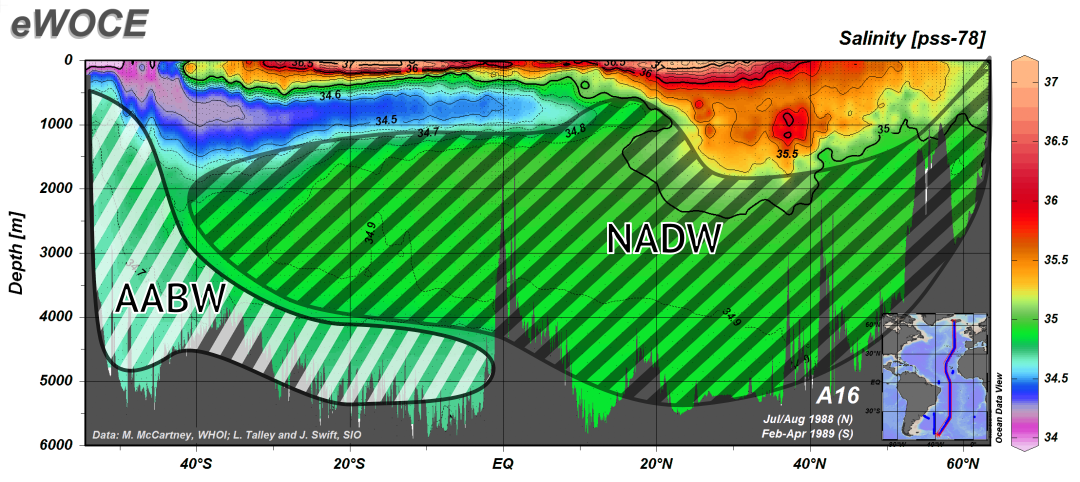
\includegraphics[width=\textwidth]{WOCE_01}
    \caption{Salinity profile of the Atlantic Ocean from  showing the distinct water masses identifiable by their salinity fingerprint. From \citet{schlitzerElectronicAtlasWOCE2000}}
    \label{fig:WOCE_01}
\end{figure}

The structure of the deep oceans is defined by the formation of deep waters in the northern and southern high latitudes as surface waters cool, gain density, and sink to the deep ocean. This process occurs in the North Atlantic Ocean, forming North Atlantic Deep Water (NADW), and in the Southern Ocean, forming Antarctic Bottom Water (AABW) and Circumpolar Deep Water (CDW) \citep{talleyChapterAtlanticOcean2011}. The very deepest parts of the South Atlantic are filled with AABW which is overlaid by NADW as it travels southwards (figure \ref{fig:WOCE_01}). The NADW is then upwelled in the Southern Ocean, where a component mixes with circumpolar waters to form CDW, and another component mixes with surface waters and is returned to the North Atlantic over the surface \citep{talleyClosureGlobalOverturning2013}. The return of this water forms the Atlantic Meridional Overturning Circulation (AMOC) cell. The strength of the AMOC has been variable in recent geological history. The AMOC may have shutdown \citep{broeckerOriginNorthernAtlantic1992} or significantly weakened \citep{oppoWhatBenthicD13C2015} during previous extreme glacial events, and may have strengthened relative to the present during the last interglacial \citep{guihouEnhancedAtlanticMeridional2011}.

In the Southern Ocean, AABW is an incredible dense water mass that forms off the coast of Antarctica, and in gaps in the ice sheet called polynyas where fast cold winds can cool the surface waters very quickly. This results in very cold, very dense waters that entrain subsurface waters as they sink \citep{ohshimaGlobalViewSeaice2016}. CDW meanwhile forms in the surrounding Southern Ocean through mixing of upwelling waters with surface waters cooled by cold circumpolar wind currents, and is (relatively) warm and saline in comparison \citep{moffatCharacteristicsCircumpolarDeep2009}. These two Southern Ocean water masses are then exported to the deep Atlantic, Pacific and Indian Oceans (figure \ref{fig:talley}).

\begin{figure}[h]
    \centering
    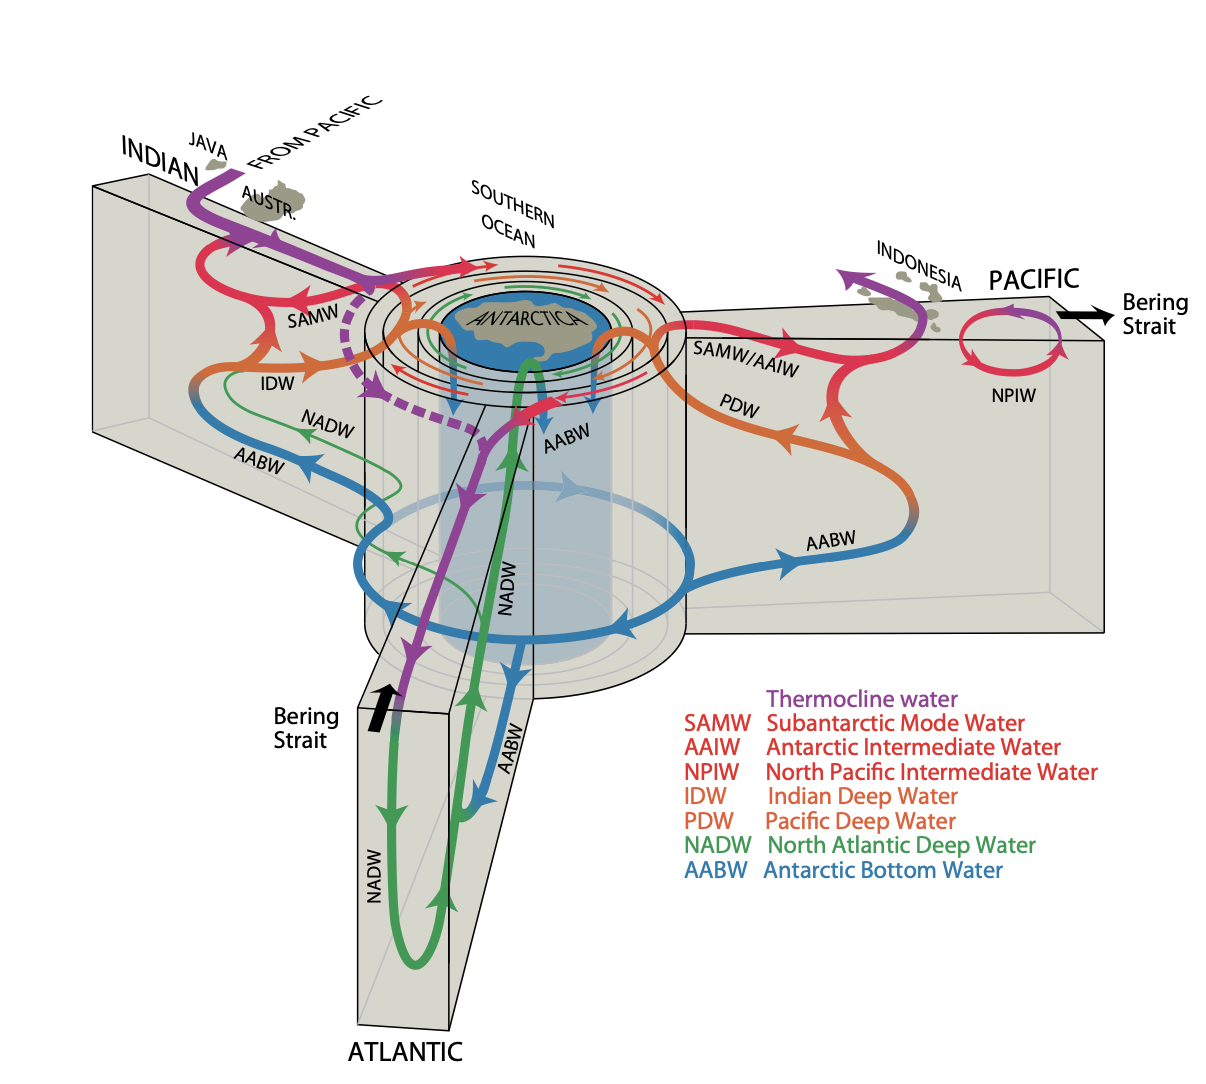
\includegraphics[width=0.8\textwidth]{talley}
    \caption{Schematic showing the paths of deep water masses around the world's oceans in the modern day. From \citet{talleyClosureGlobalOverturning2013}}
    \label{fig:talley}
\end{figure}

Unlike the Southern and Atlantic Oceans, there are no deep waters that form in the Pacific Ocean. The surface waters of the subpolar North Pacific are as cold as the North Atlantic, but are relatively fresh and this keeps them too buoyant to sink to depth \citep{warrenWhyNoDeep1983}. The deep Pacific Ocean is therefore filled by waters sourced from the Southern Ocean. This mix of CDW and AABW fill the abyssal Pacific Ocean (figure \ref{fig:WOCE_02}), where they gradually warm and mix with fresher waters to lose density, rise, and form Pacific Deep Water (PDW) \citep{talleyClosureGlobalOverturning2013}.

\begin{figure}[h]
    \centering
    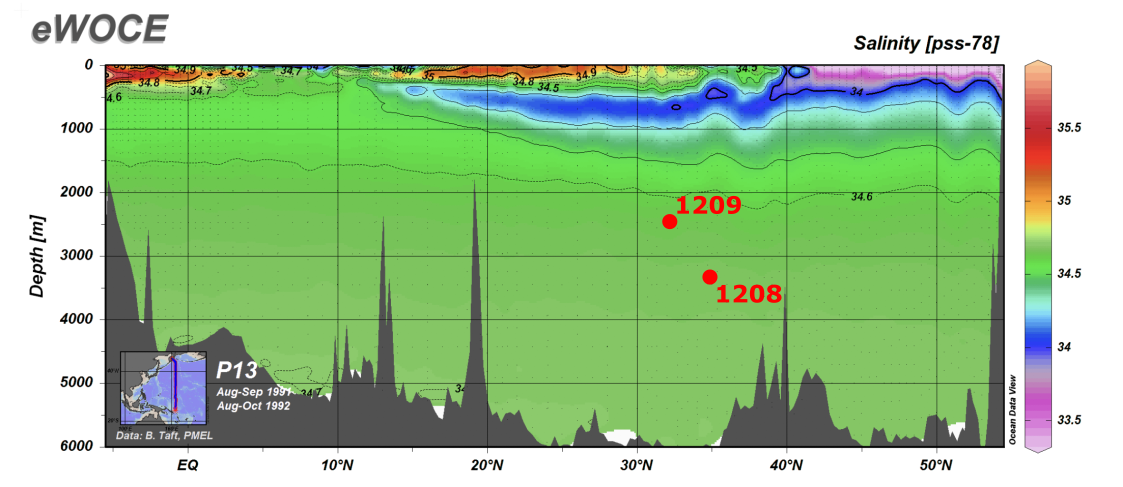
\includegraphics[width=\textwidth]{WOCE_02}
    \caption{Salinity profile of the West Pacific Ocean showing the homogeneity in deep waters below 1000 m depth. Locations of ODP Sites 1208 and 1209 are marked in red. From \citet{schlitzerElectronicAtlasWOCE2000}}
    \label{fig:WOCE_02}
\end{figure}

The strong salinity gradient in the North Pacific Ocean, or halocline, determines much of the structure of the deep Pacific Ocean. The cause of this halocline is not known, but suggestions include excess precipitation in the North Pacific \citep{stockerRapidTransitionsOcean1991}, exchange of waters from subpolar and subtropical ocean gyres \citep{emile-geayWarrenRevisitedAtmospheric2003}, and the export of fresh waters from the Atlantic to the Pacific through atmospheric teleconnections over the Isthmus of Panama \citep{richterMoistureTransportAtlantic2010}. The excess of precipitation over evaporation in the North Pacific has been attributed to moisture flux from the Asian Monsoon \citep{emile-geayWarrenRevisitedAtmospheric2003}, the shape of the Pacific Ocean basin \citep{ferreiraAtlanticPacificAsymmetryDeep2018}, or the strong SST gradient between the equatorial and subpolar Pacific Ocean \citep{burlsActivePacificMeridional2017}.


While there is no deep water formation in the North Pacific, the cold but fresh waters of the subpolar North Pacific are able to sink to form North Pacific Intermediate Waters (NPIW), which do not extend below 1000 m depth \citep{talleyDistributionFormationNorth1993}. The formation of NPIW is unusual with cool subpolar waters being forced into the East Pacific before sinking to depth \citep{youPathwayCirculationNorth2003}. NPIW is not dense enough to sink deeper than 1000 m and thus has little bearing on wider ocean circulation in the modern Pacific Ocean.


\subsubsection{Pliocene Oceanography}

In the Pliocene there are many indications that ocean circulation was fundamentally different, particularly in the Pacific Ocean. Pliocene SSTs were 2 - 3\textdegree C warmer than present and due to polar amplification, high latitude SSTs were around 10\textdegree C warmer than present \citep{wilsonPlioPleistoceneReconstructionEast2011}. This would markedly reduce the meridional (north-south) temperature gradient in the Pacific Ocean, which is been supported by SST proxies from the Pliocene \citep{fedorovTightlyLinkedZonal2015}. This reduced meridional SST gradient would decrease the amount of precipitation over the North Pacific and erode the strong halocline, which could allow for deep water formation in the Late Pliocene North Pacific \citep{burlsActivePacificMeridional2017} forming a Pacific Meridional Overturning Circulation (PMOC) cell (figure \ref{fig:burls}).

\begin{figure}[h]
    \centering
    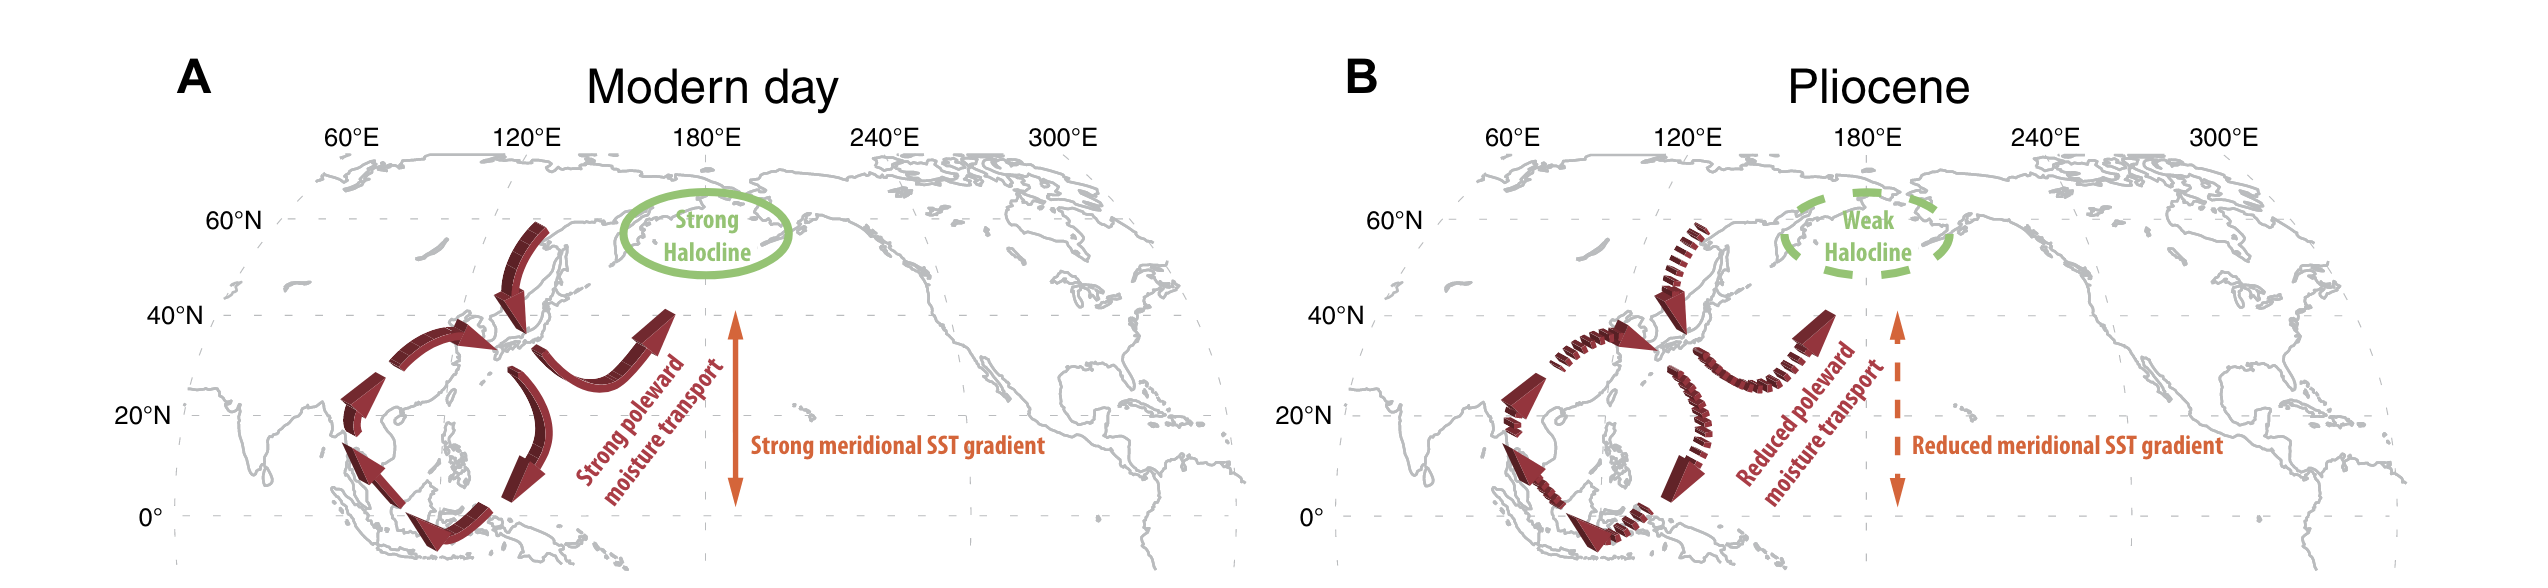
\includegraphics[width=\textwidth]{burls}
    \caption{Schematic of the impact of a reduced Pacific SST gradient in the Late Pliocene on the North Pacific halocline allowing for PMOC formation. From \citet{burlsActivePacificMeridional2017}}
    \label{fig:burls}
\end{figure}

\subsubsection{Pacific Meridional Overturning Circulation}

The presence of a Pliocene PMOC is backed up by a range of paleo-proxy evidence. High diatom productivity, indicative of a strong nutrient flux and upwelling of deep waters, is seen in the North Pacific \citep{haugOnsetPermanentStratification1999,sigmanPolarOceanStratification2004}. Upwelling waters in the North Pacific require surface waters to sink to depth to replace these, and suggest a reduced stratification in the subpolar North Pacific. This idea is supported by evidence from carbon isotopes which point to a more ventilated intermediate-depth North Pacific Ocean \citep{fordSustainedMidPlioceneWarmth2022}. The mechanism for formation of a PMOC suggests that a reduced meridional SST gradient causes reduced moisture transport to high latitudes which erodes the strong halocline in the North Pacific \citep{burlsActivePacificMeridional2017}. The removal of this halocline would allow for the formation of North Pacific Deep Waters (NPDW) which would then upwell and form this PMOC cell \citep{menvielRemovingNorthPacific2012, thomasOceanicPathwaysActive2021}. There is evidence for upwelling of nutrient-rich deep waters in the equatorial Pacific during the Pliocene \citep{shanklePlioceneDecouplingEquatorial2021} thought to be this NPDW \citep{thomasOceanicPathwaysActive2021}. The NPDW that would form from an active PMOC would be a colder, but also slightly fresher, water mass compared to the CDW and AABW water masses in the deep Pacific Ocean (figure \ref{fig:salinity}).


\begin{figure}[h]
    \centering
    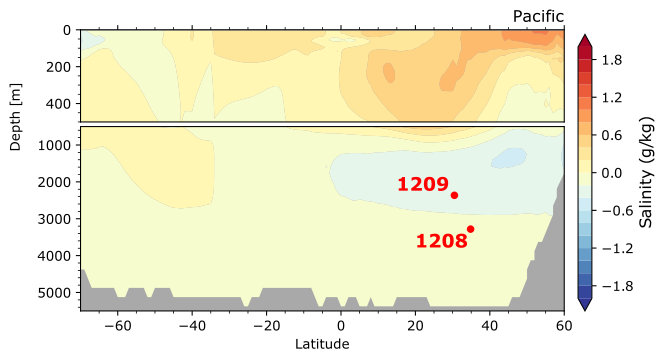
\includegraphics[width=\textwidth]{salinity}
    \caption{Model output showing salinity in the Pacific Ocean in the Late Pliocene relative to the preindustrial. Shown in red are the locations of ODP Sites 1208 and 1209. From \citet{fordSustainedMidPlioceneWarmth2022}}
    \label{fig:salinity}
\end{figure}

There is evidence that contradicts the idea of a Pliocene PMOC. Oxygen isotopes from sites in the North East Pacific Ocean show a fresher colder water mass overlying more saline waters, which could be explained by a PMOC, but also have carbon isotopes that suggest the shallower water mass was less ventilated than the deeper water mass, which does not fit with a PMOC \citep{kwiekPacificOceanIntermediate1999}. These results could be explained by the proximity of the sites to the California Margin which has occasional anoxic periods caused by high primary productivity, which would sway the carbon isotopes \citep{deanInorganicGeochemicalIndicators1997}. 

The evidence for the Pliocene PMOC is absent in the Pleistocene. North Pacific contourites, which can be used as a proxy for flow speed, suggest that deep ocean currents in the Pacific have got progressively stronger in stages since 5 Ma \citep{yinProgressiveIntensificationPacific2022}. If there was a PMOC shutdown over the iNHG, then this would decrease flow speeds in the deep Pacific Ocean, rather than have them continually increase. The contourites could be influenced by local flow factors rather than basin-wide circulation patterns or could be overprinted by erosion of the sediment which would generate inaccurate fast circulation signals \citep{stowChapterNatureContourite2008}.

Most climate models of the Late Pliocene, such as those in the PlioMIP2 model intercomparison project, are unable to generate a PMOC \citep{zhangMidPlioceneAtlanticMeridional2021,haywoodPlioceneModelIntercomparison2020}. It is possible to generate a PMOC in a climate model but this requires changing the forcings to remove the North Pacific halocline \citep{burlsSimulatingPlioceneWarmth2014, burlsActivePacificMeridional2017, menvielRemovingNorthPacific2012}. This indicates that there is no well-described mechanism for why a PMOC might form. Theoretical ocean models of the Pacific Ocean have event suggest that the shape of the Pacific Ocean, particularly the width of the Pacific basin relative to the Atlantic, would make it impossible for a PMOC to ever form \citep{jonesSizeMattersAnother2017,jonesInterbasinTransportMeridional2016}. The lack of a PMOC in climate models of the Late Pliocene does not explain the evidence for strong overturning in the North Pacific. Furthermore, there is evidence from the last glacial period of significant deep water formation in the North Pacific. Radiocarbon ventilation ages in the North Pacific show a marked drop down to 2700 m depth in the last deglaciation indicative of a sinking of NPIW to depths far beyond what is possible in the modern day \citep{okazakiDeepwaterFormationNorth2010}. Neodymium and boron isotopes in the North Pacific corroborate this idea of an expanded intermediate or even deep water mass in the extending down to as far as 3400 m depth \citep{raeDeepWaterFormation2014}, and as far south as the Australian Coast \citep{struveDeepTasmanOutflow2022}. The suggestion of deep circulation in the Pacific for both past glacials and the Late Pliocene implies that there is no fundamental block to deep circulation, but this is instead a factor of a strong halocline in the modern North Pacific Ocean.

\subsubsection{Atlantic Circulation}

The warmer world of the Pliocene is thought to have had stronger overturning circulation and a greater export of NADW out of the North Atlantic \citep{raymoMidPlioceneWarmthStronger1996, raveloEnhancedCirculationWarm2000}. There is strong evidence for a greater NADW in the Pliocene from carbon isotopes in the Southern Atlantic \citep{raymoResponseDeepOcean1992} and neodymium isotopes in the mid-Atlantic \citep{frenzCarbonatePreservationPatterns2006}. Alkenone and planktic foraminiferal proxies show a reduced meridional SST gradient in the North Atlantic and a reduced nutrient content from an invigorated North Atlantic current, which is indicative of a stronger AMOC \citep{naafsLatePlioceneChanges2010, karasPlioceneOceanicSeaways2017}. These results are supported by climate model outputs which point to a faster and more active overturning in the Atlantic during the warm Late Pliocene \citep{weiffenbachUnravelingMechanismsImplications2022}.

\subsection{Influence of the iNHG on Ocean Circulation}

\subsubsection{Cessation of the PMOC}

The evidence of a PMOC that comes from carbon isotopes and opal production is absent after the iNHG \citep{haugNorthPacificSeasonality2005, swannSalinityChangesNorth2010}. This is accompanied by evidence from diatoms of a strong subpolar North Pacific halocline established at 2.73 Ma \citep{swannDiatomD18OEvidence2006, studerEnhancedStratificationSeasonality2012}, which would suppress any deep water formation. The reason why this halocline forms is disputed.

A stronger halocline could be the result of global atmospheric cooling over the iNHG. This would increase the meridional SST gradient in the Pacific Ocean due to greater cooling at the poles than at the equator \citep{fedorovTightlyLinkedZonal2015} and result in greater net precipitation in the North Pacific, strengthening the halocline \citep{brierleyRelativeImportanceMeridional2010, burlsActivePacificMeridional2017}. The stronger halocline could also be the result of large ice sheets terminating in the Bering Sea and the Gulf of Alaska. These would bring a supply of freshwater to the North Pacific which could strengthen the halocline, as has been suggested for the last glacial period \citep{praetoriusRoleNortheastPacific2020}. However, the first IRD evidence for marine-terminating ice sheets in Alaska is only found after 2.65 Ma \citep{maslinProgressiveIntensificationNorthern1996}, approximately 100 ka after the establishment of a permanent North Pacific halocline.

The establishment of a halocline may also have been driven by tectonic forcings. The final closure of the Central American Seaway (CAS) separating North and South America occurred by 2.7 Ma. This can be seen in fossil evidence for the exchange of vertebrate species between the two continents \citep{molnarClosingCentralAmerican2008}. The coincident timing of the closure of the CAS and the cessation of the PMOC could imply a link. Climate models have suggested that with the closure of the seaway, warm and saline waters from the Caribbean Sea and the Gulf of Mexico would be transported to the North Atlantic rather than the North Pacific, freshening the surface North Pacific \citep{brierleyComparingImpactsMiocene2016}. However, while the final closure of the CAS occurred at 2.7 Ma, the seaway was likely closed to deep water transport much earlier. Evidence from neodymium isotopes suggest the seaway may have closed as early as 10 Ma \citep{sepulchreConsequencesShoalingCentral2014}, though most other evidence suggests that significant water mass transport through the CAS was stopped by 5-3 Ma \citep{molnarClosingCentralAmerican2008}. These timings suggest that the closure of the CAS is unlikely to play a role in the cessation of the PMOC over the iNHG.

Modelling evidence has also pointed to the importance of the Bering Strait in modulating salinity in the North Pacific \citep{huPacificAtlanticSeesawBering2012, otto-bliesnerAmplifiedNorthAtlantic2017}. The Bering Strait currently allows for the export of fresh waters out of the Pacific Ocean into the North Atlantic \citep{huBeringStraitThroughflow2005}. Closure of these straits would result in a freshening of the North Pacific and strengthen the subpolar North Pacific halocline. There is evidence for the first shallow opening of the Bering Strait from 5.3 Ma \citep{gladenkovRefinedAgeEarliest2002}, but it would be closer to 4.8 Ma before there was significant exchange of water through the strait \citep{marincovichEvidenceEarlyOpening1999}. The shallowness of the Bering Strait means that only 0.8 Sv is transport through the strait in the present day \citep{huRoleBeringStrait2012}, but climate models have shown that this can have a major effect on deep ocean circulation \citep{brierleyComparingImpactsMiocene2016, otto-bliesnerAmplifiedNorthAtlantic2017}. The shallowness of the Bering Strait means that this process is also highly dependent on sea level \citep{huInfluenceBeringStrait2010}. The sea level fluctuations over the iNHG could therefore have played a key role in suppressing the PMOC.

It seems likely that the PMOC is shutdown over the iNHG due to the establishment of a strong halocline in the North Pacific. However, the response of the deep Pacific Ocean to this halocline is poorly understood. Understanding the causes of, and responses to, the decline of the PMOC would also aid in our understanding of the mechanisms that were driving it.

\subsubsection{Wider Oceanographic Changes}

Outside the changes to the PMOC, the iNHG sees some wider oceanographic changes in the Pacific and Atlantic Oceans. There is evidence from Mg/Ca ratios in benthic foraminifera which show a convergence in bottom-water temperatures (BWT) between the deep Atlantic and Pacific Oceans over the iNHG \citep{woodardAntarcticRoleNorthern2014}. This convergence in water mass properties between the deep Pacific and Atlantic Oceans might be the result of ice sheet and sea ice growth on Antarctica \citep{woodardAntarcticRoleNorthern2014}. The expanded Antarctic ice sheet would result in more CDW formation and export to both the Atlantic and Pacific Oceans, resulting in a more homogenous, ``Antarctic'', BWT signal in both oceans \citep{hillModelledOceanChanges2017}. Carbon and oxygen isotopes from the Plio-Pleistocene point to the presence of two distinct southern-sourced water masses in the South Atlantic over the iNHG, which may represent CDW water masses sourced from different parts of Antarctica \citep{vanderweijstTernaryMixingModel2020}. The convergence of the BWT signals in the North Pacific and Atlantic Oceans could be the result of a PMOC shutdown, and a weaker AMOC, which would result in a more “Southern Ocean” signal in both oceans without the need for stronger CDW export. The accuracy of the North Atlantic BWT estimates has also been questioned due to the influenced of local carbonate ion saturation \citep{yuCommentDeepSeaTemperature2010,sosdianResponseCommentDeepSea2010,sosdianDeepSeaTemperatureIce2009}.

Alternatively, a stronger AMOC in the North Atlantic over the iNHG could result in more NADW-like BWT signal being exported to the Pacific Ocean after the iNHG \citep{kwiekPacificOceanIntermediate1999}. Proxy studies from the North Atlantic indicate that AMOC strength may have increased over the iNHG \citep{hayashiLatestPlioceneNorthern2020}. However, there is evidence from carbon and neodymium isotopes in the mid and South Atlantic that AMOC strength is weakened over the iNHG \citep{hodellHighResolutionStableIsotopic1992, langIncursionsSouthernsourcedWater2016}, which would undermine this theory. 

\subsection{Oceanographic Techniques}

Understanding how ocean circulation has changed requires the ability to trace past water masses. This can be done through a variety of proxies for water mass characteristics. Carbon and oxygen isotopes in foraminifera can tell us about the productivity, salinity, and temperature of past water masses. The trace metal ratios of foraminiferal tests are able to indicate how the temperature and carbon state of water masses changed over time. These proxies tell us about water mass properties that are generally well conserved by water masses as they travel through the oceans. This allows them to be used as identifiers of distinct water masses \citep{kimOriginTsushimaCurrent2005, raeDeepWaterFormation2014, woodardAntarcticRoleNorthern2014}. Neodymium isotopes can be used to show the provenance of different water masses \citep{amakawaNeodymiumIsotopicVariations2004}. The original signals in all of these proxies are prone overprinting by local signals and thus are often used in conjunction with each other to get a clearer picture of past ocean circulation.

\subsubsection{Oxygen Isotopes and Salinity}
\label{sec:oxygen}

Oxygen (and carbon) isotopes have been one of the most important techniques in oceanography dating back to the 1950s. The ratio of the stable isotopes of oxygen, $^{18}$O and $^{16}$O, in the carbonate tests of foraminifera can be used to infer the temperature of formation of the test as well as giving an indication of the global ice volume \citep{crissPrinciplesStableIsotope1999}. This is often denoted by $\delta^{18}\text{O}$ which is defined as:

\begin{align}
\delta^{18}\text{O}=\left(\frac {\left(\frac {^{18}\text{O}}{^{16}\text{O}}\right)_{\text{sample}} }{\left({\frac {^{18}O}{^{16}\text{O}}}\right)_{\text{standard}}}-1\right)\times 1000
\end{align}

The lighter isotopes of oxygen are preferentially fractionated into water vapour, and not into precipitation, resulting in lighter isotopes preferentially travelling to higher latitudes \citep{raveloChapterEighteenUse2007}. As these lighter isotopes are then preferentially trapped in ice sheets, this allows the resultant oxygen isotope ratio of sea water to reflect the global ice volume \citep{shackletonOxygenIsotopesIce1987}. The formation of calcite from seawater by foraminifera further fractionates these oxygen isotopes, with the degree of fractionation controlled by the temperature of the surrounding seawater \citep{raveloChapterEighteenUse2007}. Therefore, $\delta^{18}$O measurements from foraminifera can broadly be used as a proxy for local temperature and global ice volume. 

\begin{figure}[h]
	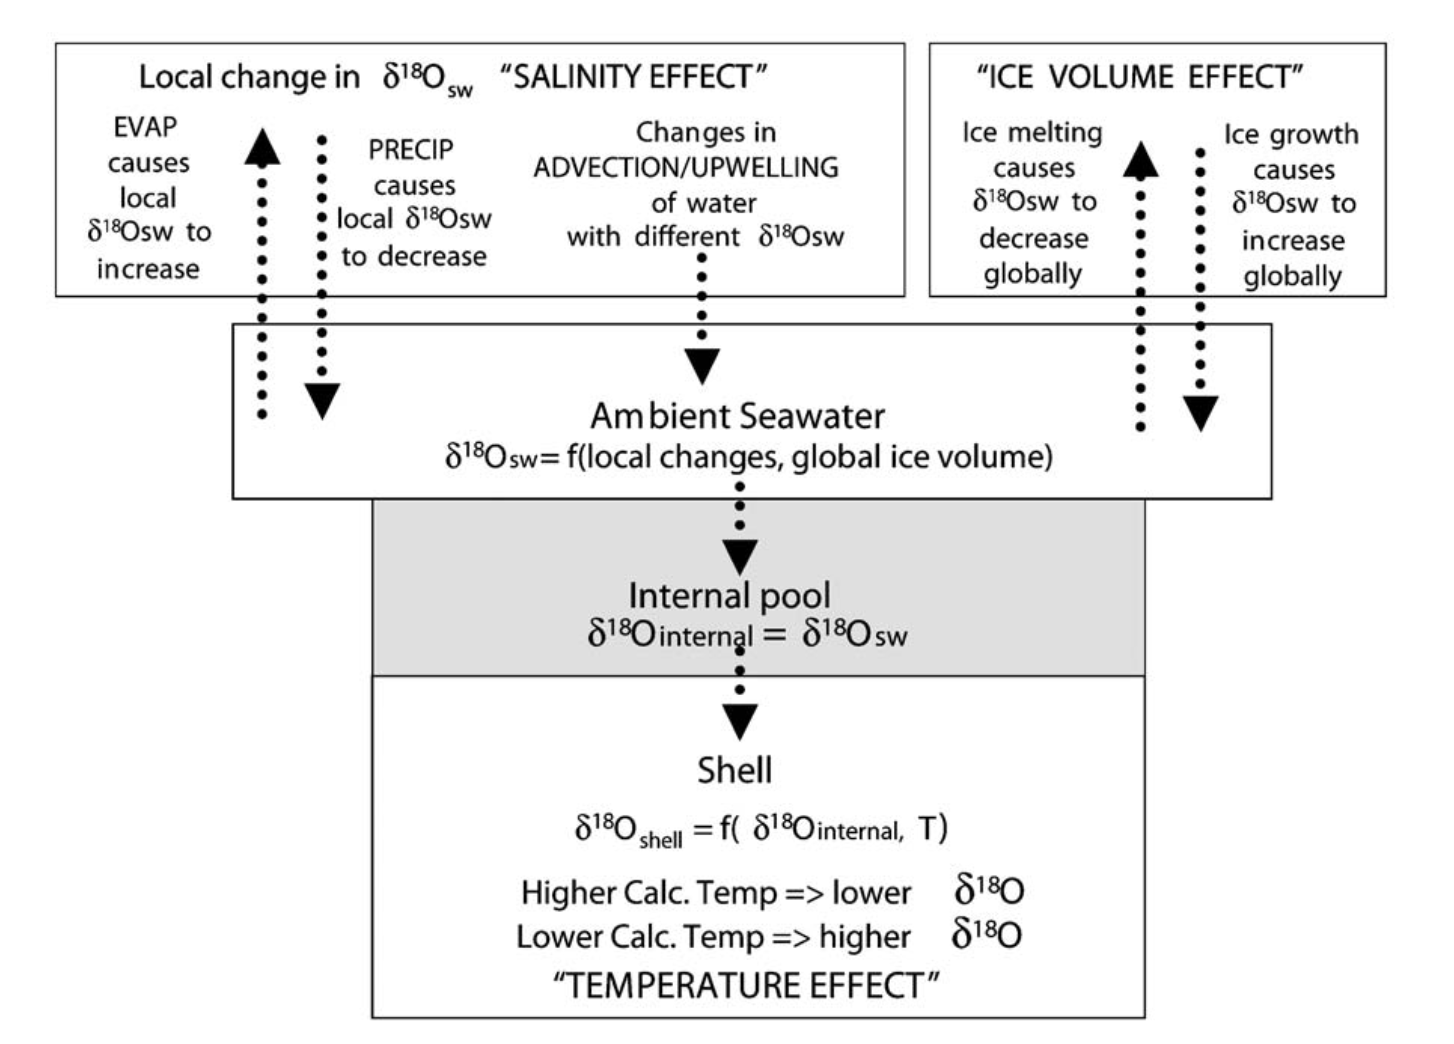
\includegraphics[width=0.9\textwidth]{d18O}
	\centering
	\caption{Environmental factors that influence the $\delta^{18}\text{O}$ of calcite in benthic foraminifera. From \citet{raveloChapterEighteenUse2007}}
	\label{fig:d18O}
\end{figure}

There are many more smaller effects that can affect the resultant $\delta^{18}\text{O}$ of foraminiferal calcite (figure \ref{fig:d18O}). The most important of these is the ``salinity effect'', where local precipitation causes changes to both the salinity and $\delta^{18}\text{O}$ values of the seawater \citep{benwayOxygenIsotopesUpperocean2004}. The surface salinity is then conserved as these surface waters sink to form deep waters, allowing oxygen isotopes to act as a proxy for salinity, and a water mass tracer.

As $\delta^{18}\text{O}$ measures both local temperature and salinity of water masses, it can be thought of as a proxy for density \citep{guAssessingAbilityZonal2019}. Higher $\delta^{18}\text{O}$ values correspond to colder or more saline water masses, and therefore also more dense waters. However, it is possible to decouple $\delta^{18}\text{O}$ values from density through processes such as sea ice formation, which reject brine from formation but do not fractionate oxygen isotopes \citep{gebbieMeridionalCirculationLast2006}. In the South Atlantic there is evidence of waters with higher $\delta^{18}\text{O}$ values sourced from the North Atlantic overlying lower $\delta^{18}\text{O}$ Southern Ocean waters \citep{lynch-stieglitzMeridionalOverturningCirculation2006} which is thought to represent the impact of sea ice formation on generation of very cold deep waters off the coast of Antarctica \citep{toggweilerEffectSeaIce1995}. While the correlation between $\delta^{18}\text{O}$ values and salinity is generally only applicable at very small scales \citep{conroyConstraintsSalinityOxygen2014}, the use of oxygen isotopes as a salinity proxy can still be useful - particularly if coupled with an independent measure of bottom-water temperatures.

\subsubsection{Magnesium Calcium Ratios and Bottom Water Temperatures}
\label{sec:mgca}

The ratio of Mg$^{2+}$ to Ca$^{2+}$ ions in calcite has been used as a proxy for past ocean temperatures in the tests of corals \citep{rossCalibrationSrCa2019}, ostracods \citep{rodriguez-tovarTraceFossilsEvidence2019}, and planktic \citep{hollandConstrainingMultipleControls2020} and benthic \citep{barrientosArcticOceanBenthic2018} foraminifera. The advantage of this method compared to other palaeothermometers such as alkenones is the ability to measure ambient temperatures around benthic foraminifera, and thus determine bottom water temperatures.

The principle of Mg/Ca ratios in foraminifera is that foraminiferal tests are built of calcite, CaCO$_3$, but the Ca$^{2+}$ ion can be substituted for Mg$^{2+}$ ion to form MgCO$_3$. This substitution is an endothermic reaction and thus is favoured at higher temperatures \citep{elstnerovaInitioStudyThermodynamic2010}. In a completely inorganic system, it is possible to determine the degree of Mg substitution using the enthalpies of formation of MgCO$_3$ and CaCO$_3$, which should increase exponentially with temperature \citep{rosenthalTemperatureControlIncorporation1997}. However, in biogenic calcite, there are significant vital controls on this process, resulting in much lower but also much more temperature dependent Mg$^{2+}$ incorporation into calcite \citep{martinQuaternaryDeepSea2002, bentovImpactBiomineralizationProcesses2006}. This biogenic control on the incorporation of Mg$^{2+}$ ions could be achieved through amorphous secondary phases from which calcite tests grow, involvement of an organic matrix to filter out unwanted ions, or pumping ions out of the parent solution to reduce local Mg$^{2+}$ concentrations \citep{bentovImpactBiomineralizationProcesses2006, erezSourceIonsBiomineralization2003}. Nano-scale x-ray spectroscopy points to continuous incorporation of Mg$^{2+}$ into foraminiferal calcite suggesting that it is likely that the calcite grows in one phase and therefore that we can still use linear or exponential relationships between temperature and Mg/Ca despite these vital effects \citep{bransonCoordinationMgForaminiferal2013}. However, these vital effects can differ between species, and occasionally between morphotypes, of foraminifera \citep{steinkeMgCaRatios2005, schmittSingleForaminiferaMg2019}.

To determine a temperature of shell formation from the Mg/Ca ratio requires species specific calibrations between formation temperature and Mg/Ca ratios. While planktic foraminifera can be grown in a laboratory setting \citep{grayNonthermalInfluencesMg2019} to study the non-thermal influences on Mg/Ca and determine the temperature calibration, for benthic species the only way to do this is through core-top studies \citep{lea14ElementalIsotopic2014}. Core-top studies from benthic foraminifera are able to come up with region specific as well as species specific calibrations, such as this calibration for Uvigerina peregrina in the tropical Pacific Ocean \citep{stirpeMgCaProxy2021}. The relationship between Mg/Ca and temperature varies between exponential and linear relationships for different species and temperature ranges (figure \ref{fig:mgca}) \citep{elderfieldCalibrationsBenthicForaminiferal2006}.


\begin{figure}[h]
	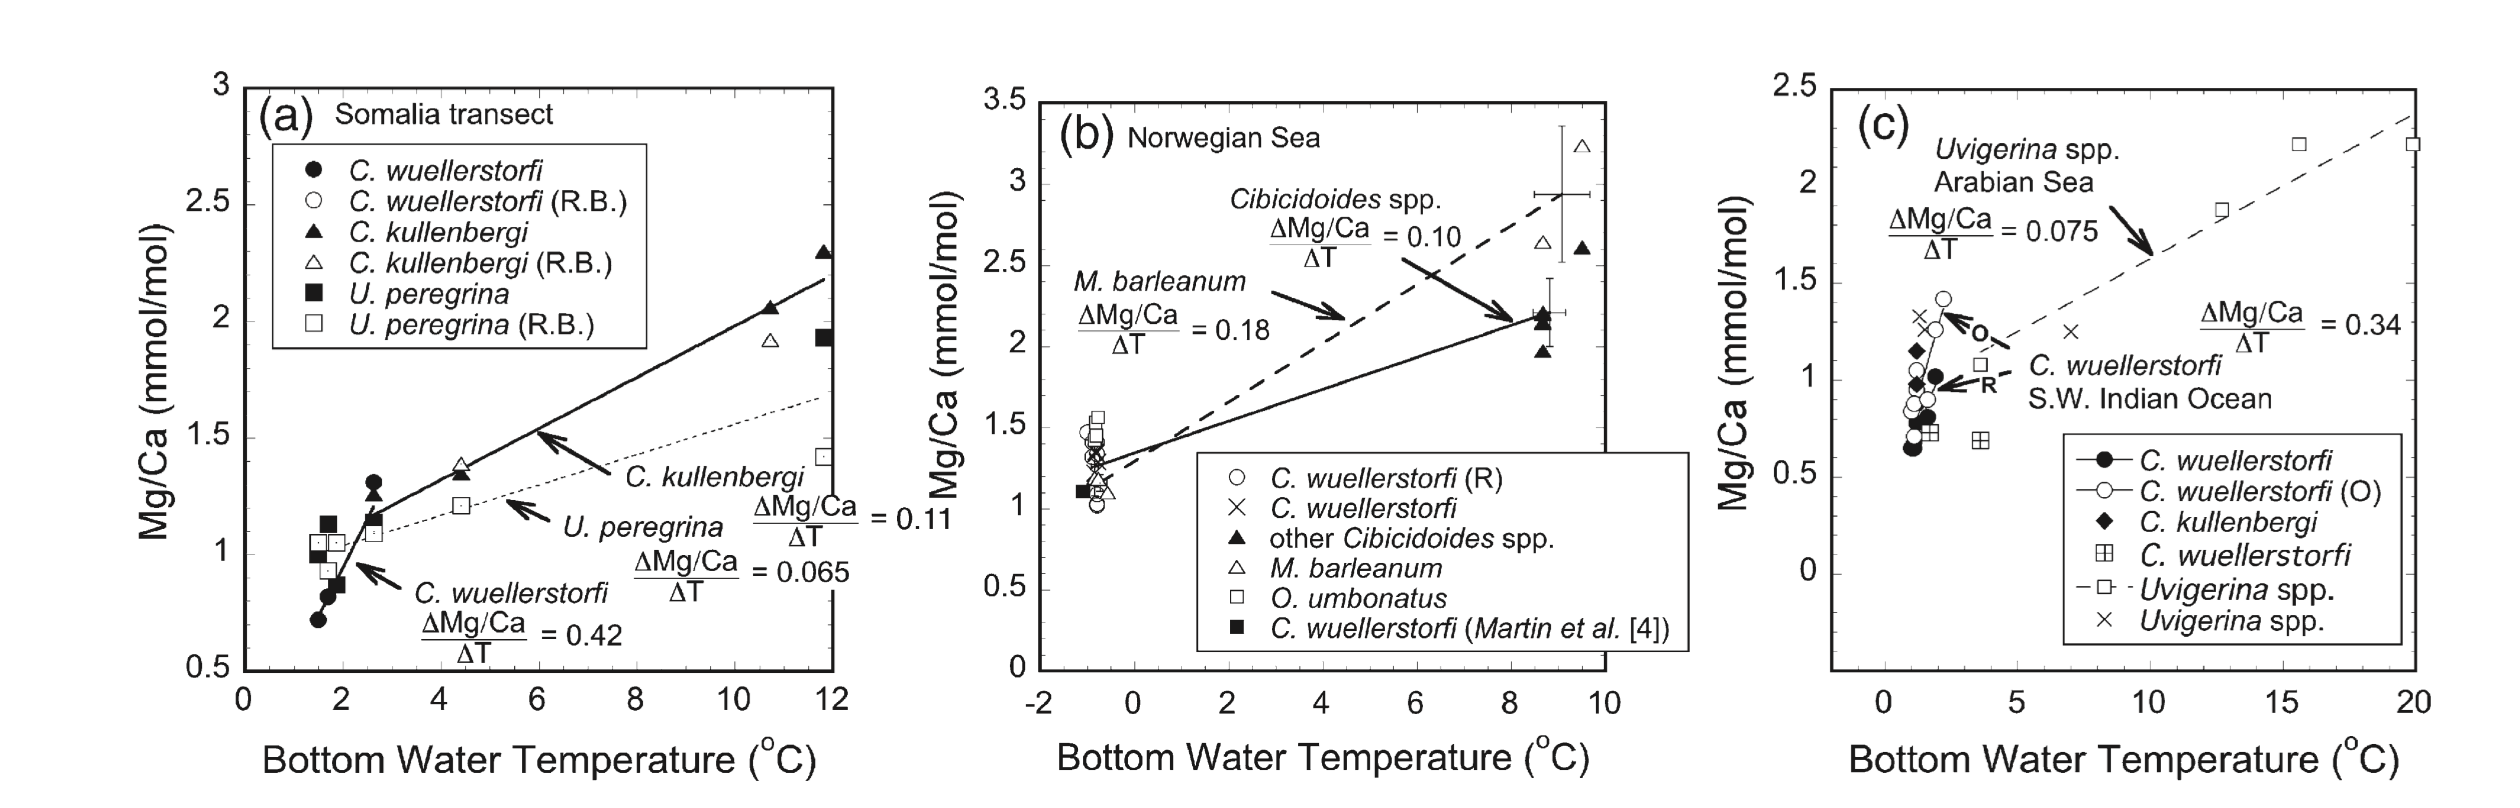
\includegraphics[width=0.9\textwidth]{mgca}
	\centering
	\caption{Mg/Ca-BWT calibrations for benthic foraminifera species from different ocean basins. From \citet{elderfieldCalibrationsBenthicForaminiferal2006}}
	\label{fig:mgca}
\end{figure}

There are a variety of non-thermal controls on Mg/Ca incorporation into calcite. There are suggestions that Mg/Ca ratios can decrease with increasing water depth \citep{lea14ElementalIsotopic2014} and salinity \citep{dissardImpactSalinityMg2010}. The problem with Mg/Ca is that Mg$^{2+}$ concentrations are often very low, with concentrations of less than 0.3\% by weight \citep{emilianiMineralogicalChemicalComposition1955}, and therefore dissolution of part of a calcite shell can have marked changes on resultant Mg/Ca ratios \citep{barkerStudyCleaningProcedures2003}. There are suggestions that Mg$^{2+}$ enriched sections of calcite tests are more prone to dissolution compared to normal calcite, which would preferentially lower Mg/Ca ratios with increased dissolution \citep{brownVariationsMgCa1996}. 

Carbonate ion concentration, $\Delta\left[ \text{CO}_{3}^{-} \right]$, also has a control on Mg/Ca ratios in certain benthic foraminifera \citep{rosenthalTemperatureCarbonateIon2006}. Most notably, the Mg/Ca ratios from \emph{Cibicidoides wuellerstorfi}, a species often used for oxygen and carbon isotope studies, has been shown to be independent of temperature, and solely dependent on $\Delta\left[ \text{CO}_{3}^{-} \right]$ \citep{yuMgCaBenthic2008}. Selection of specific benthic foraminifera species, such as \emph{Uvigerina} \citep{elderfieldCalibrationsBenthicForaminiferal2006}, or \emph{Oridorsalis umbonatus} \citep{learNeogeneIceVolume2015}, which are not affected by $\Delta\left[ \text{CO}_{3}^{-} \right]$ is therefore required to obtain reliable BWT estimates.

A final control on Mg/Ca ratios is the Mg/Ca ratio of the seawater (Mg/Ca$_\text{sw}$), which can bias temperature reconstructions \citep{lea14ElementalIsotopic2014}. The residence time of Mg$^{2+}$ in the oceans, $\sim$10 Myr \citep{hemStudyInterpretationChemical1985}, is much longer than the age of the iNHG, and thus the Mg/Ca$_\text{sw}$ is unlikely to have changed markedly since the Pliocene. Evidence to suggest that the Mg/Ca$_\text{sw}$ was around 5.2 mol mol$^{-1}$ during the mPWP, compared to the present value of 3 - 4 mol mol$^{-1}$ \citep{evansPlankticForaminiferaShell2016}. Assuming Mg/Ca$_\text{sw}$ has linearly decreased from the Pliocene to the present, it is possible to correct Pliocene Mg/Ca ratios for this Mg/Ca$_\text{sw}$ offset \citep{evansPlankticForaminiferaShell2016, jakobNewSealevelRecord2020}.

Even with the correct species of foraminifera and corrections for non-thermal factors, Mg/Ca measurements are prone to error from contamination. Accurate Mg/Ca measurements therefore rely thorough oxidative and reductive cleaning of foraminifera samples prior to measurement \citep{boyleComparisonAtlanticPacific1985, barkerStudyCleaningProcedures2003}. The reductive cleaning steps can result in dissolution of sample and lower Mg/Ca ratios \citep{elderfieldCalibrationsBenthicForaminiferal2006, yuPreferentialDissolutionBenthic2007}, but are shown to remove most contaminants that could influence the final result \citep{weldeabComparisonForaminiferalCleaning2006}. 

The strength of Mg/Ca as a proxy is beyond just accurate BWT estimates. As deep-water temperatures only change when they are exposed to the surface or through mixing with other water masses, Mg/Ca derived BWT can be used as a semi-conservative water mass tracer \citep{woodardAntarcticRoleNorthern2014, jakobDeepoceanCirculationNorth2021}. As explained earlier, the $\delta^{18}\text{O}$ composition of benthic foraminiferal tests ($\delta^{18}\text{O}_\text{benthic}$) is a measure of both local BWT and the $\delta^{18}\text{O}$ of seawater ($\delta^{18}\text{O}_\text{sw}$). Mg/Ca is an independent measure of BWT, allowing coupled Mg/Ca-$\delta^{18}\text{O}$ measurements to resolve the temperature dependence of $\delta^{18}\text{O}_\text{benthic}$ to give the $\delta^{18}\text{O}_\text{sw}$ at the time of formation of the test, and therefore more accurate estimates of global ice volume \citep{elderfieldEvolutionOceanTemperature2012, raymoAccuracyMidPlioceneD18Obased2018}. The difference between the global average $\delta^{18}\text{O}_\text{sw}$ and local $\delta^{18}\text{O}_\text{sw}$ is a function of regional hydrological changes \citep{gonfiantiniStableIsotopeFractionations2020}, allowing coupled Mg/Ca-$\delta^{18}\text{O}_\text{benthic}$ measurements to be used as a paleo-salinity proxy in planktic foraminifera \citep{flowerPhasingDeglacialWarming2004,  schmidtLinksSalinityVariation2004, nurnbergInteractingLoopCurrent2008}.


\subsubsection{Boron Calcium Ratios and Carbonate Ion Concentrations}
\label{sec:baca}

The ratio of boron to calcium in calcite can be used as a proxy for the carbonate ion saturation of seawater \citep{honischBoronProxiesPaleoceanography2019}. This is based on the idea that boron, or more specifically borate, $\text{B(OH)}_{4}^{-}$, can be incorporated into calcite in place of carbonate:

\begin{align}
\text{CaCO}_{3_{\text{solid}}} + \text{B(OH)}^{-}_{4_{\text{aq}}} \leftrightarrow \text{CaHBO}_{3_{\text{solid}}} + \text{HCO}^{-}_{3_{\text{aq}}} + \text{H}_{2}\text{O}_{\text{aq}}
\end{align}

The B/Ca ratio should then be a function of the concentration of boron, $\left[\text{B}_{\text{T}}\right]$, and bicarbonate, $\left[\text{HCO}_{3}\right]$, in seawater \citep{yuBenthicForaminiferalCa2007}. Empirical studies of core-top conditions and B/Ca ratios show a strong relationship between B/Ca in calcite and $\Delta\left[ \text{CO}_{3}^{-} \right]$ \citep{yuBenthicForaminiferalCa2007, raeBoronIsotopesCa2011}. The relationship between B/Ca and $\Delta\left[ \text{CO}_{3}^{-} \right]$ is dependent on species, and sometimes even morphotypes within species (figure \ref{BCa}), suggesting a strong physiological control on boron incorporation into foraminiferal calcite \citep{raeBoronIsotopesCa2011}.

\begin{figure}[h]
	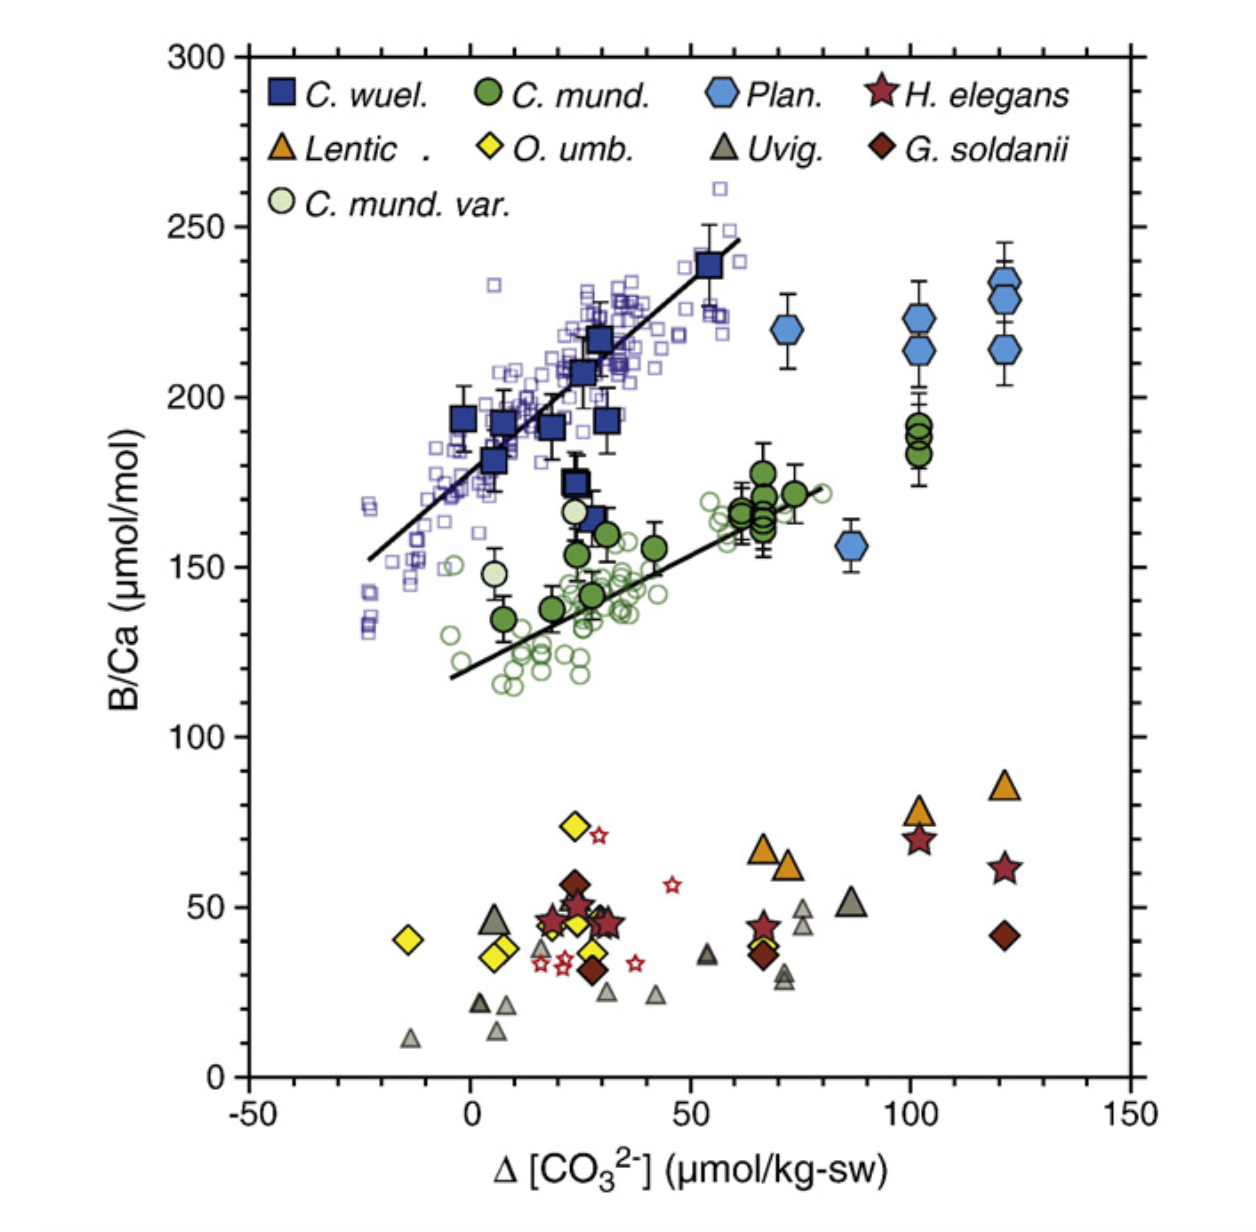
\includegraphics[width=0.9\textwidth]{BCa}
	\centering
	\caption{Relationship between B/Ca and $\Delta\left[ \text{CO}_{3}^{-} \right]$ for various benthic foraminifera species and morphotypes of \emph{C. mundulus}. From \citet{raeBoronIsotopesCa2011}}
	\label{BCa}
\end{figure}

The $\Delta\left[ \text{CO}_{3}^{-} \right]$ describes the difference between the bottom water carbonate concentration and the saturation concentration at that location:

\begin{align}
\Delta\left[ \text{CO}_{3}^{-} \right] = \left[ \text{CO}_{3}^{-} \right]_{\text{in situ}} - \left[ \text{CO}_{3}^{-} \right]_{\text{saturation}}
\end{align}

The $\left[ \text{CO}_{3}^{-} \right]_{\text{saturation}}$ is a function of the depth, pressure, and salinity \citep{lynch-stieglitz16TracersOcean2004}. Knowledge of these water mass properties allows us to estimate the $\left[ \text{CO}_{3}^{-} \right]$ of seawater \citep{yuBenthicForaminiferalCa2007}. While the depth of a particular site is often known for at least the last 10 million years, the salinity, and thus $\left[ \text{CO}_{3}^{-} \right]_{\text{saturation}}$, of past water masses can only be reliably estimated for a few hundred thousand years \citep{honischBoronProxiesPaleoceanography2019}. For further into deep time, B/Ca carbonate reconstructions require estimates of past salinity, which could be derived from coupled Mg/Ca-$\delta^{18}$O measurements (see section: \ref{sec:mgca}) and estimates of seawater boron concentration \citep{tripatiCouplingCO2Ice2009}.

Using B/Ca ratios to estimate past carbonate concentration can be influenced by the boron concentration in seawater \citep{uchikawaInfluenceSolutionChemistry2017,uchikawaExperimentalEvidenceKinetic2015}. The residence time of boron in the oceans is between 10 and 20 Myr \citep{crumpton-banksBoronIsotopesProvide2020}. This means that total boron concentration in seawater is not believed to have changed considerably on Pliocene timescales, and the total boron concentration can be effectively modelled for this timescale \citep{lemarchandInfluenceRiversMarine2000, lemarchandBoronIsotopeSystematics2002}.


The ocean carbonate system can be defined by 4 independent equations with 6 components \citep{irvingCARBONICACIDCARBONATEEQUILIBRIUM1925}, shown below:

\begin{align}
	\text{CO}_2 + \text{H}_2\text{O} &\leftrightarrow \text{H}_2\text{CO}_3 \\
	\text{H}_2\text{CO}_3 &\leftrightarrow \text{HCO}_3^- + \text{H}^+ \\
	\text{HCO}_3^- + \text{H}^+ &\leftrightarrow \text{CO}^{2-}_{3} + 2 \text{H}^{+} \\
	\text{H}_2\text{O} &\leftrightarrow \text{H}^+ + \text{OH}^-
\end{align}

Therefore, if two of these components are known it is possible to infer the state of the carbonate system at this location. B/Ca provide knowledge of one of these components, $\left[ \text{CO}_{3}^{-} \right]$, but requires another measurement to determine the whole system. This could be $\delta^{11}$B measurements to infer past pH \citep{fosterSeawaterPHPCO22008}, or modelling past carbonate ion ratios \citep{tripatiCouplingCO2Ice2009} to solve this issue.

Knowledge of the carbonate concentration of deep-waters can be used to infer carbon storage in the abyssal oceans allowing for estimates of past atmospheric CO$_2$ concentrations \citep{tripatiCouplingCO2Ice2009, chalkDynamicStorageGlacial2019}. B/Ca ratios can also be used to estimate the circulation of carbon through an ocean reservoir \citep{yuSeawaterCarbonateIond13C2008, yuDeepOceanCarbonate2014}. As carbonate concentration in deep-waters only changes with surface exchange or through mixing with other water masses, it is also possible to use B/Ca as a semi-conservative water mass tracer akin to $\delta^{13}$C measurements \citep{chalkDynamicStorageGlacial2019}.

\subsubsection{Neodymium Isotopes as a water mass tracer}

Seeing how the strength of deep water formation has changed over time can be most easily achieved through examining the spatial extent of water masses. All else being equal, a stronger AMOC would result in a greater NADW extent, while a weaker PMOC would result in a reduced NPDW extent. The relative proportions of isotopes of neodymium (Nd) within the authigenic fraction of ocean sediments provides an archive of past seawater compositions which can be translated into an estimate of water mass extent. 

Since Nd isotopes, and specifically $^{143}$Nd and $^{144}$Nd, do not fractionate within sediments \citep{bizimisNeodymiumIsotopes2016}, the difference in isotope concentrations is primarily due to the decay of $^{147}$Sm into $^{143}$Nd \citep{lugmairSmNdAgesNew1974}. Samarium is slightly less incompatible than neodymium during mantle melting, so the Sm/Nd ratio in mantle melts is lower than in the mantle residue. This residue forms continental rocks which then have a lower Sm/Nd ratio, and over time this will result in a lower $^{143}$Nd/$^{144}$Nd ratio compared to igneous rocks \citep{bizimisNeodymiumIsotopes2016}. The ratio of neodymium isotopes is often expressed as $\varepsilon_\text{Nd}$, the ratio of $^{143}$Nd/$^{144}$Nd relative to the bulk silicate Earth \citep{goldsteinLonglivedIsotopicTracers2003} as below:

\begin{align}
\varepsilon_\text{Nd} = \left[ \left\{ \frac{(^{143}\text{Nd}/^{144}\text{Nd})_\text{sample}}{(^{143}\text{Nd}/^{144}\text{Nd})_\text{bulk Earth}}\right\} -1 \right]\times10^4
\end{align}

Older cratonic rocks will have negative $\varepsilon_\text{Nd}$ values, while younger volcanic rocks will have positive values \citep{lambeletNeodymiumIsotopicComposition2016}. As these rocks are weathered, the physical products end up as sediments in the ocean. The Nd that is released in dissolved form retains the $\varepsilon_\text{Nd}$ value of the original sediments and imparts this signature to the ocean. Therefore, water masses surrounded by younger rocks, such as the Pacific Ocean, usually have more positive $\varepsilon_\text{Nd}$ values compared to those found in the North Atlantic Ocean \citep{goldsteinLonglivedIsotopicTracers2003}. This is supported by modern observations of seawater composition (figure \ref{fig:nd_map}).

\begin{figure}[h]
	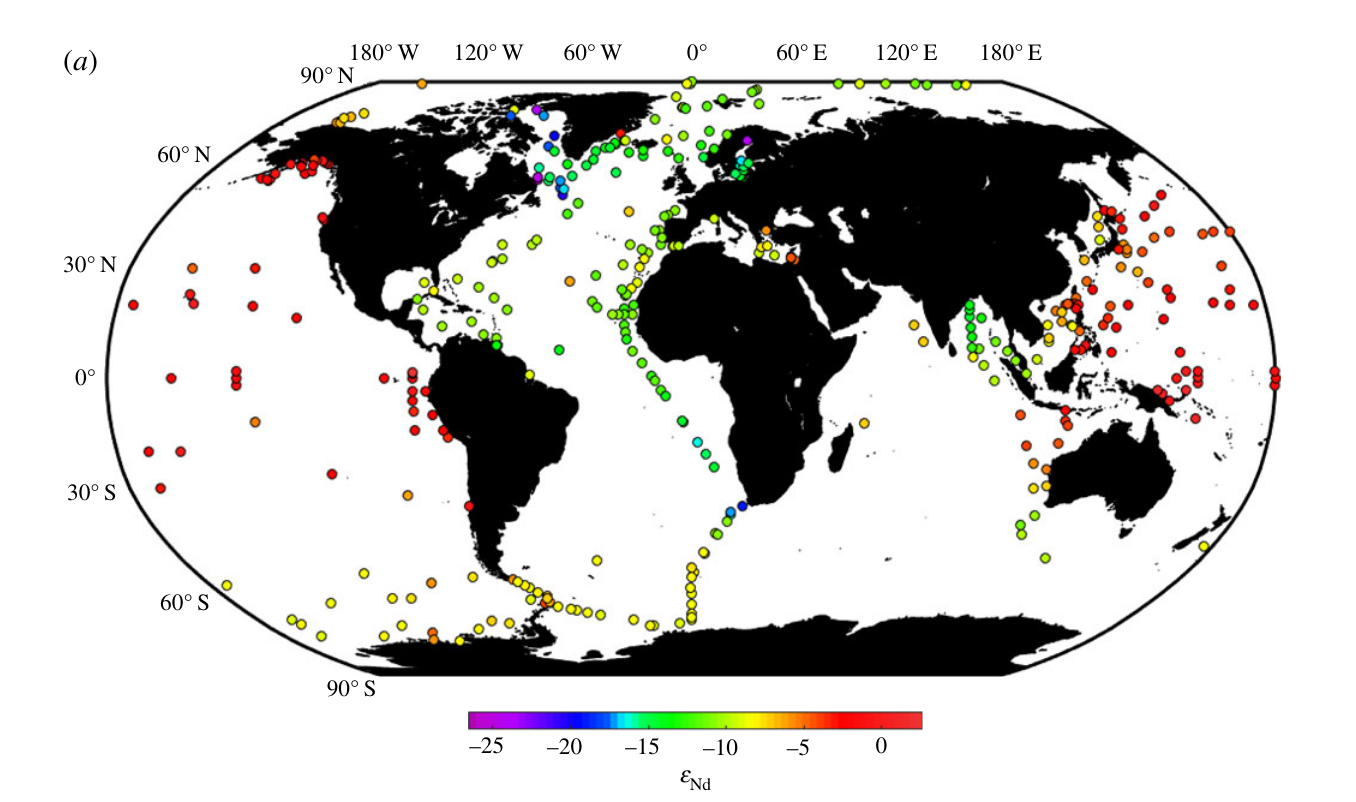
\includegraphics[width=0.9\textwidth]{nd_map}
	\centering
	\caption{Map of modern seawater $\varepsilon_\text{Nd}$ values from ocean cruises, many of which were conducted as part of the GEOTRACES project \citep{vandeflierdtNeodymiumOceansGlobal2016}}
	\label{fig:nd_map}
\end{figure}

Deep water formation only occurs in a few specific places \citep{gebbieHowOceanFilled2011}. The surface water $\varepsilon_\text{Nd}$ value at these deep water formation sites determines the eventual deep waters that form. The residence time of Nd in the oceans is about 200 - 1000 years \citep{tachikawaNewApproachNd1999}, and shorter than the overturning time of the oceans. This means that Nd is not well mixed in the oceans, but varies spatially, which can be used to trace water mass origins \citep{bizimisNeodymiumIsotopes2016}. 

The Nd isotope composition of deep waters can be recorded in authigenic sediments that precipitate out of seawater. Commonly used archives include fish teeth \citep{osborneSeawaterNeodymiumLead2014}, corals \citep{vandeflierdtTemporalStabilityNeodymium2006}, and foraminifera \citep{tachikawaNeodymiumAssociatedForaminiferal2014}. Coupled with accurate age models, these Nd records can show how relative proportions of water masses have changed over time at certain locations.

Determining the provenance of past water masses from $\varepsilon_\text{Nd}$ measurements requires a knowledge of past end member $\varepsilon_\text{Nd}$ compositions, the $\varepsilon_\text{Nd}$ values for the surface waters. This is well constrained for the modern day \citep{vandeflierdtNeodymiumOceansGlobal2016}, but may have changed in the past in ways that are difficult to model (figure \ref{fig:model_nd}).

\begin{figure}[h]
	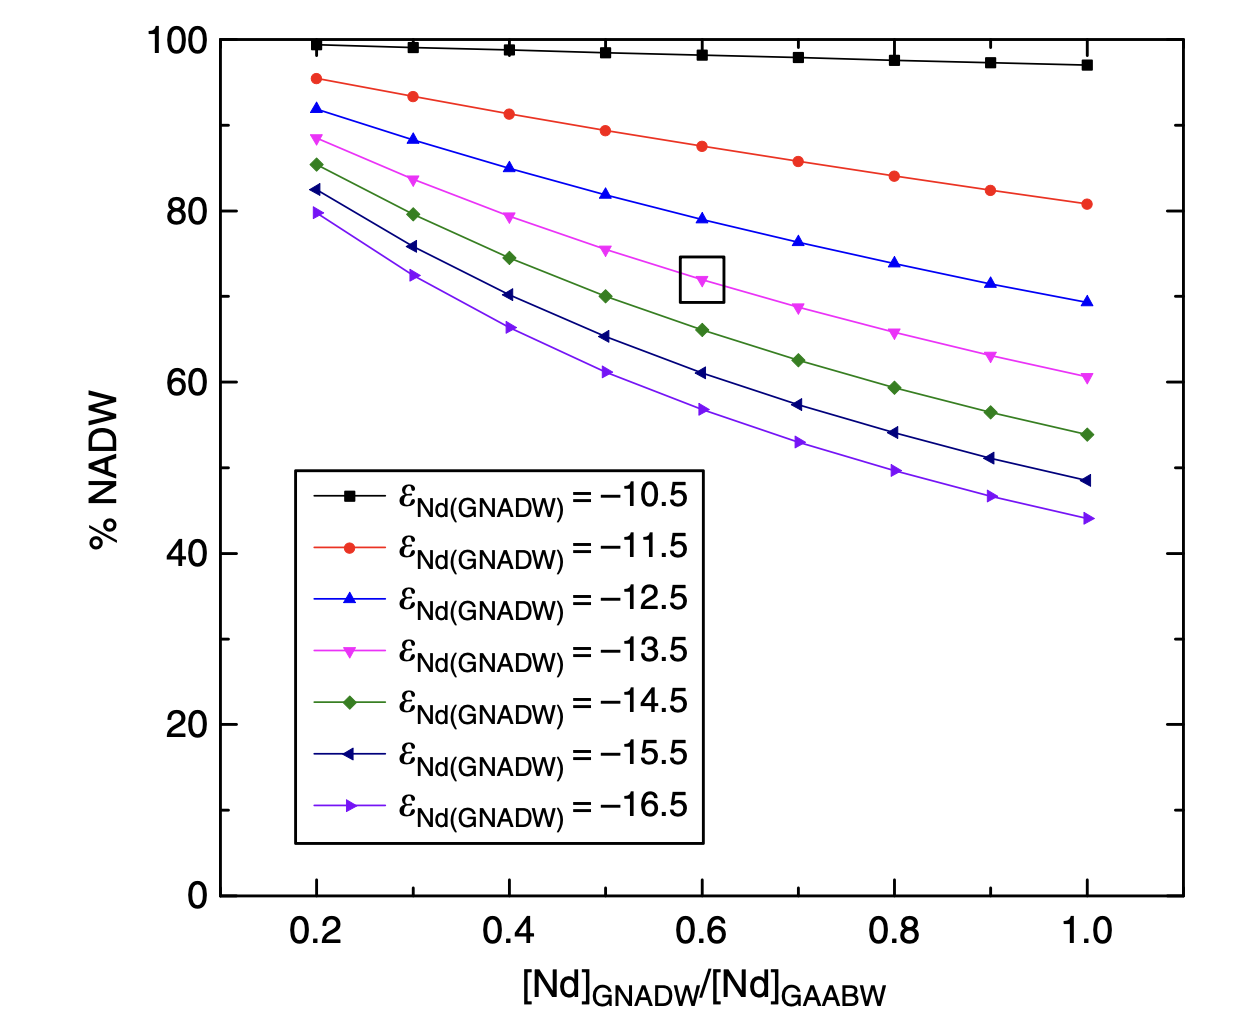
\includegraphics[width=0.9\textwidth]{model_nd}
	\centering
	\caption{Estimates of the percentage of NADW at a site in the deep North Atlantic during the Last Glacial Maximum for a range of different end-member NADW $\varepsilon_\text{Nd}$ compositions and Nd concentrations \citep{howeNorthAtlanticDeep2016}}
	\label{fig:model_nd}
\end{figure}

Determining past circulation patterns based on estimates of endmember $\varepsilon_\text{Nd}$ values is further complicated by the fact that deep water masses have not always have formed in the same places as today. How relative contributions of ISOW, DSOW, and LSW to deep waters forming in the North Atlantic has changed in the past is still poorly constrained for the last glacial limiting the effectiveness of $\varepsilon_\text{Nd}$ as a tracer of water mass extent \citep{dokkenRapidChangesMechanism1999, hillaire-marcelAbsenceDeepwaterFormation2001, crocketPersistentNordicDeepwater2011, larkinActiveNordicSeas2022}. When coupled with other semi-conservative water mass tracers, such as oxygen isotopes, Mg/Ca, and B/Ca measurements, $\varepsilon_\text{Nd}$ measurements can be used to deconvolve the relative contributions of these components of deep water masses. 

Even if we could perfectly model the formation of past deep water masses, reconstructing circulation through $\varepsilon_\text{Nd}$ measurements still faces several hurdles. Simple interpretations of water mass mixing based on $\varepsilon_\text{Nd}$ rely on Nd behaving as a conservative element within the oceans, despite the evidence to suggest otherwise \citep{lacanNeodymiumIsotopesNew2005, jeandelOverviewMechanismsThat2016, jeandelIsotopicNdCompositions2007, haleyImpactBenthicProcesses2017}. This is primarily due to boundary exchange and benthic flux.

Particles are able to scavenge Nd from the water column, which removes the total Nd concentration in the oceans in a process referred to as boundary exchange \citep{jeandelOverviewMechanismsThat2016}. This does not directly affect the $\varepsilon_\text{Nd}$ value but makes seawater $\varepsilon_\text{Nd}$ values more prone to isotopic shifts caused by the transport of continental-derived sediments to the deep ocean which can then dissolve and change deep ocean $\varepsilon_\text{Nd}$. This is benthic flux \citep{duNeodymiumIsotopesAuthigenic2016, abbottBottomsSedimentaryControl2015}. Together these two processes can markedly change seawater $\varepsilon_\text{Nd}$ values. The effects of benthic flux and boundary exchange can be limited through empirical modelling of sedimentary fluxes within the ocean \citep{haleyImpactBenthicProcesses2017, poppelmeierNeodymiumIsotopesPaleowater2022}.

Neodymium isotopes can be used to determine the extent of water masses in the ocean, which can be used to infer the strength of overturning circulation cells, such as the AMOC or PMOC. The extent of water masses such as NADW is not only a factor of AMOC strength but also export of Southern Ocean deep water masses which limits how much can be inferred from these isotopes in isolation \citep{langIncursionsSouthernsourcedWater2016}. In combination with flow speed proxies, such as sortable silt, or Pa/Th, it may be possible to infer past overturning strength \citep{jonkersDeepCirculationChanges2015}.

\subsection{The Impact of the iNHG on Volcanism}

\subsubsection{The Interaction between Volcanism and the Climate}

Volcanic eruptions are the result of tectonic plate movements on geological timescales. Plate movements allow cracks to develop in the Earth’s lithosphere, through which magma can rise. As it does so, the lower pressure melts the magma resulting in volcanism. This volcanism can play a major role in shaping the Earth’s climate by releasing greenhouse gases and aerosols into the atmosphere \citep{hayTectonicsClimate1996, kenderPaleoceneEoceneCarbon2021}. This can occur on the annual timescales for sulphate aerosols \citep{zhuPersistingVolcanicAsh2020}, or multi-millennial timescales or longer for CO$_2$ emissions and changes to the carbon cycle \citep{siglTimingClimateForcing2015, lohmannIceCoreEvidence2022}. The influence of volcanism on the climate highlights the importance of understanding the triggers for volcanism. 

Volcanism can have an impact on the climate, but it is also possible for climate shifts to influence rates of volcanism. This is predominately done through the movement of ice sheets which place large stresses on the lithosphere \citep{nakadaIceAgeTrigger1992}. Rates of volcanism on Iceland were found to be considerably higher during the end of the last glacial than during the period before or after \citep{maclennanLinkVolcanismDeglaciation2002}. This is linked to the removal of the ice sheet over Iceland following the deglaciation resulting in a reduction of pressure on the crust, increasing the rate of magma melting and thus volcanism \citep{aubryImpactClimateChange2022}. This relationship is less straightforward with arc volcanism potentially due to deeper magma chambers \citep{wattVolcanicResponseDeglaciation2013}. There is also a suggestion that sea level changes can influence volcanism through increased stress on mid-ocean ridges \citep{boulahanisSeaLevelVariations2020}. On longer timescales, it is possible to observe pulses in the rates of volcanism which correspond to orbital timescales, suggesting that volcanism may be influenced by ice sheets outside the last deglacial \citep{schindlbeckMioceneHoloceneMarine2018}.

\subsubsection{The Influence of the iNHG on Volcanism}

The iNHG represents an increase in ice volume across much of the Northern Hemisphere. The increased loading from ice sheets could result in a reduction in the eruption rate due to greater stress on the lithosphere increasing the pressure on the magma chamber and thus reducing melting. Alternatively, compared to the lack of Pliocene ice sheets in the Northern Hemisphere \citep{hillCharacterizingIceSheets2007}, the rapidly retreating and advancing ice sheets of the Pleistocene could induce volcanism through fracturing of the crust and allowing more paths for magma to ascend and then melt. Therefore, it would be the rate of change of ice volume rather than the removal of ice volume that could influence the eruption rate \citep{jellinekDidMeltingGlaciers2004}. It has been suggested that the increased volcanism in Eastern California during Pleistocene interglacials may have been triggered by ice advance \citep{glaznerFireIceAnticorrelation1999}. This increased fracturing of the crust could also lead to more dyke emplacement allowing for release of pressure from the magma chamber prior to eruption, reducing the rate of eruptions \citep{sigmundssonClimateEffectsVolcanism2010}. At the scale of single volcanoes, the shape of individual magma chambers can introduce significant heterogeneities in the rates of magmatism \citep{sigmundssonMultipleEffectsIce2012}.

Evidence does suggest that there is increased volcanism in the Pleistocene compared to previous epochs which could be the result of increased ice sheet loading \citep{kennettGlobalIncreaseQuaternary1975}. However, this may also be an artefact of greater preservation of more recent sediments \citep{hawkesworthMatterPreservation2009}. 

Previous studies have yet to look at the impact of the iNHG on volcanism.  There is an increase in tephra layers recorded in North Pacific sediments around 2.65 Ma \citep{prueherRapidOnsetGlacial1998, prueherVolcanicTriggeringLate2001}, which occurs before the appearance of IRD, evidence of widespread glaciation. This suggests that locally to the North Pacific, volcanism may have been a cause, rather than an effect, of the increased glaciation \citep{prueherRapidOnsetGlacial1998}. There is evidence from the North Atlantic suggesting an increase in tephra layers in the Late Pliocene, potentially linked to the growing ice sheets \citep{lacasseEnhancedAirborneDispersal2002}. There is no synchronous increase in terrestrial deposition of tephra on Iceland over the Late Pliocene \citep{geirsdottirGrowthIntermittentIce1994} indicating that this increase may not be the result of an increased rate of volcanism.

\subsubsection{Changes in the Rate of Volcanism}

Determining past changes in rates of volcanism measured in the accumulation of tephra. Tephra describes siliciclastic ejecta from volcanic eruptions, layers of which can be buried in the sediment and become part of the stratigraphy. Greater numbers of tephra layers can be used as an indicator of increased volcanism \citep{kutterolfMilankovitchFrequenciesTephra2019}. Geochemical analysis of tephra layers allows layers to be tied to specific volcanic eruptions \citep{bourneTephraLatticeGreenland2015}, or magmatic processes \citep{maclennanLinkVolcanismDeglaciation2002}, allowing for inferences on the causes of change of rates of volcanism.

Tephra analysis in marine sedimentary sequences, either visually or geochemically, requires the extraction of vitreous glass shards from the sediment \citep{blockleyNewLessDestructive2005}. Tephra is made of predominately volcanic glasses, which are prone to dissolution, removing all visible traces of the original tephra layer. Observations of cryptotephra layers, layers which contain so few glass shards that they are invisible to the naked eye, can partially counter this problem \citep{daviesCryptotephrasRevolutionCorrelation2015}. Cryptotephra analysis allows for the detection of much smaller tephra concentrations, revealing tephra at greater distances from volcanic sources \citep{wastegardEvidenceOccurrenceVedde1998, mckayAntarcticSouthernOcean2012}. Volcanic glass shards within tephra layers are also prone to dissolution by laboratory processes \citep{blockleyNewLessDestructive2005}. Extraction of tephra shards through a stepped floatation protocol rather than by use of acid washing of sediments can limit the laboratory influences on tephra shards \citep{blockleyNewLessDestructive2005}. Comparison of multiple proximate cores can be used to correct for the local effects of dissolution \citep{abbottTracingMarineCryptotephras2018}.

Tephra layers are prone to reworking, particularly by the tectonic forces that produce the tephra in the first place \citep{nakayamaDepositionalProcessesPrimary1997}, leading to the development of inaccurate stratigraphies through misidentification of primary deposits \citep{hopkinsDepositionPreservationTephra2020}. These problems can be partially overcome through analysis of many proximate sites \citep{abbottTracingMarineCryptotephras2018}, and through modelling tephra reworking \citep{hopkinsDepositionPreservationTephra2020}.













